% ****** Start of file aipsamp.tex ******
%
%   This file is part of the AIP files in the AIP distribution for REVTeX 4.
%   Version 4.1 of REVTeX, October 2009
%
%   Copyright (c) 2009 American Institute of Physics.
%
%   See the AIP README file for restrictions and more information.
%
% TeX'ing this file requires that you have AMS-LaTeX 2.0 installed
% as well as the rest of the prerequisites for REVTeX 4.1
% 
% It also requires running BibTeX. The commands are as follows:
%
%  1)  latex  aipsamp
%  2)  bibtex aipsamp
%  3)  latex  aipsamp
%  4)  latex  aipsamp
%
% Use this file as a source of example code for your aip document.
% Use the file aiptemplate.tex as a template for your document.

\RequirePackage{graphicx} % this line is required to see pics in draft mode
\documentclass[%
 aip,
 draft,
% jmp,
% bmf,
% sd,
% rsi,
 amsmath,amssymb,
%preprint,%
 reprint,%
%author-year,%
%author-numerical,%
% Conference Proceedings
]{revtex4-1}

\usepackage{graphicx}% Include figure files
\usepackage{dcolumn}% Align table columns on decimal point
\usepackage{bm}% bold math
%\usepackage[mathlines]{lineno}% Enable numbering of text and display math
%\linenumbers\relax % Commence numbering lines
\usepackage{hyperref}
\usepackage[utf8]{inputenc}
\usepackage[T1]{fontenc}
\usepackage{mathptmx}
\usepackage{amsmath}
\usepackage{multirow}
\usepackage{makecell}
\usepackage[inline, nomargin]{fixme}
\usepackage{physics}

\graphicspath{{Pictures/}}
\begin{document}

\preprint{AIP/123-QED}

\title[Automated analysis of single-tone spectroscopic data of cQED systems]{Automated analysis of single-tone spectroscopic data of cQED systems\\~}
% Force line breaks with \\

\author{G.Fedorov}
\email{gleb.fedorov@phystech.edu}

\affiliation{ 
Russian Quantum Center, Skolkovo village, Russia
}%
\affiliation{ 
Moscow Institute of Physics and Technology, Dolgoprudny, Russia
}%

\author{A. Ustinov}
\affiliation{ 
Russian Quantum Center, Skolkovo village, Russia
}%
\affiliation{%
Karlsruhe Institute of Technology, Karlsruhe, Germany
}%

\date{\today}% It is always \today, today,
             %  but any date may be explicitly specified

\begin{abstract}
Physical systems for quantum computation require calibration of the control parameters based on their physical characteristics by performing a chain of experiments that gather more and more precise information about the given device. It follows that there is the need for automatic data acquisition and interpretation. In this work, we have developed a tool that allows automatic analysis of single-tone spectroscopy (STS) results for a single qubit-resonator cell in the cQED architecture. Using several analytic approaches and maximum likelihood estimation, our algorithm is able to find all of the physical characteristics using only the STS data. It is fast and robust to noise, and its Python implementation is ready to be used with transmon qubits coupled to notch-port resonators.
\end{abstract}

\maketitle

 \renewcommand*{\figureautorefname}{Fig.}

\section{Introduction} \label{sec:level1} 

Computation on a quantum computer involves operating large numbers of physical quantum bits (qubits). One of the most significant challenges in the domain is that qubit systems cannot be operated identically:\cite{kelly2018, chen2018} typically, control parameters for a device depend on its physical parameters and are determined by a sequence of calibration experiments. Since the devices cannot be produced identical, the optimal parameters vary among them and should be found \textit{in situ}. Manual tuning of these parameters is not a scalable solution, and operating just a few dozens of qubits already requires a computer system to handle the calibration on its own. Moreover, a lot of research is still being done to optimize chip designs and fabrication methods. This research includes gathering statistics on many different samples that should be measured and consistently evaluated. An automated measurement system not only will speed up this process, but as well exclude human error.

In this work, we are proposing and implementing several methods of data processing and computer vision that aid automatic calibration of circuit QED\cite{blais2007} architectures used to read out the quantum states of superconducting qubits. Computer vision is understood here as an enterprise that employs statistical methods to disentangle data using models constructed with the aid of geometry, physics, and learning theory.\cite{forsyth2011} As it will be shown below, the outputs of circuit calibration on certain steps have to be represented as images, and it is hardly possible to automatically extract the required information from them without resorting to methods of computer vision. The proposed approach is accurate, fast and robust to noise, applicable to superconducting qubits with a periodic spectrum described with a closed form model equations, and compatible with the paradigm of one readout resonator per one qubit.\cite{versluis2017, kelly2015}

In this paradigm, the flow of an experiment that characterizes a single qubit-resonator cell of a quantum processor chip is depicted schematically in \autoref{fig:detection}(a). It is similar to the  procedures described in Refs. [\onlinecite{jerger2013, chen2018}] for measuring cQED samples with qubits of tunable frequency. For non-tunable qubits, a different algorithm of automatic calibration was described in the patent application Ref. [\onlinecite{bloom2018}]. 

We now briefly discuss each step shown in \autoref{fig:detection}(a). Usually, one starts by locating the frequency of the resonance dip in the transmission corresponding to the resonance frequency of the readout resonator. Having found the dip, the experimenter knows the scan range to set for the probe frequency $f_p$ during the next step: single-tone spectroscopy (STS). STS tracks the frequency shift of the resonance dip while changing the magnetic field applied to the sample (controlled by some current $I$). By processing the results of the STS, one can get a coarse estimate on the qubit frequency dependence on $I$  denoted as  $f^{(0)}_{ge}(I)$ (one gets as well accurate estimates on the resonator frequency $f_r(I)$ and the resonator-qubit coupling strength $g$). Based on these results, one may set the scan ranges for the excitation frequency and the current ($f_{exc}$ and $I$) for the two-tone spectroscopy (TTS). Finally, by processing the TTS result, one can obtain the precise dependence of the qubit transition frequency  $ge$ on current $f_{ge}(I)$	 with accuracy sufficient for pulsed experiments. In overall, the process is structured so that the results of one measurement step define the parameters of the next, successively acquiring more accurate information about the physical system.

\begin{figure*}
	\centering
	\includegraphics[width=0.95\linewidth]{detection_sts}
	\caption{(a) \fxnote{(a) replace 'seach' with 'seaRch' above}A common experiment flow to calibrate a tunable-frequency qubit: usually, the single- and two-tone spectroscopic measurements are performed before pulsed experiments, and each next experiment is based on the results of the previous. (b) Examples of the desired outputs (lower row) for three types of qualitatively different STS data (upper row). The 2D heatmaps should be brought into correspondence with 1D model curves. In the first column, the so called avoided crossing pattern is shown where two model curves $f_+(I)$ and $f_-(I)$ have to be fitted simultaneously since the model is discontinuous (the qubit transition frequency $f_{ge}(I)$ may be tuned both above or below the bare resonator frequency $f_c$). Conversely, the second and the third heatmaps should be described by a single continuous curve: it is $f_+(I)$ for the former (where $f_{ge}(I)<f_c;\ \forall I$) and $f_-(I)$ for the latter ($f_{ge}(I)>f_c;\ \forall I$).}
	\label{fig:detection}	
\end{figure*} 

As one can see, the results that are obtained in this scheme may be divided in two groups: some contain single curves (data are 1D manifolds), and others contain heatmap images (2D manifolds). The scope of this work is confined to the automatic analysis of the latter; precisely, we are interested in STS data processing. In \autoref{fig:detection}(b) we illustrate three types of correlated measured data and the theoretical model: depending on the qubit-resonator disposition, we desire that STS data are interpreted as either a single curve or two curves defined by the model. Precisely, we are aiming at building a method that is able to distinguish between these three cases and to estimate quantitatively the physical parameters of the system based on best-fitting model. 

The model should be based on the theoretical description of the cQED systems and physical qubits; therefore, in Appendices \ref{sec:transmon} and \ref{sec:cqed} we derive all the necessary equations to form the model curves that are expected to appear in single-tone spectroscopy. We use a transmon\cite{koch2007} with an asymmetric SQUID (superconducting quantum interference device) as a qubit; however, since our methods do not depend on the particular shape of the qubit energy levels, for other types of qubits the logic will stay the same and there is no loss of generality.

For the singe-tone spectroscopy, they model curves are (see \autoref{fig:detection}(b)):
\begin{align}
f_\pm(I) \equiv f_r(I) = \frac{f_c + f_{ge}(I)}{2} \pm \sqrt{g^2+(f_{ge}(I) - f_c)^2/4},\label{eq:f_r}
\end{align}
where $f_c$ stands for the current-independent \fxnote*{What is bare cavity frequency? Is it related to the frequency of the resonance dip of the readout resonator?}{bare cavity frequency.} Here we note again that for the avoided crossings pattern both curves are necessary; alternatively, for the cases when the qubit is entirely below (above) the bare cavity frequency only $ f_+(I)\ \left(f_-(I)\right)$ is used. Finally, the qubit transition $f_{ge}(I)$ is expressed as
\begin{equation}
f_{ge}(I) = f_{ge}^{max} \left[\cos^2\left(\frac{\pi(I-I_{ss})}{\Pi}\right)+d^2 \sin^2 \left(\frac{\pi(I-I_{ss})}{\Pi}\right)\right]^\frac{1}{4},
\label{eq:tr_spectrum}
\end{equation}
where $\Pi$ is the period of the spectrum in current, $d$ is the SQUID asymmetry and $f_{ge}^{max}$ is the qubit frequency at the sweet spot current $I = I_{ss}$, where the external magnetic field exactly compensates the non-zero local field that is always present on the chip in experiment.

In overall, we have 6 parameters for our model: $f_c$, $g$, $\Pi$, $I_{ss}$, $f_{ge}^{max}$ and $d$. Since they are in fact the parameters in the Hamiltonian for the compound cavity-qubit system as described in Appendix \ref{sec:transmon}, hereafter we call them the Hamiltonian parameters.

The structure of the rest of the paper is as follows. First, we describe our approach to extract the Hamiltonian parameters from the STS data. Next, the accuracy, performance and reliability of the algorithm is addressed; finally, we discuss the limitations of the algorithm, further applications and future work. 



\section{Methods}

Before describing the used methods, we first highlight important peculiarities of the data itself and some essential experimental details. A sample in the cQED architecture is usually studied in terms of how it interacts with incident microwave radiation. Therefore, the standard mathematical concept to describe its properties is the scattering matrix $S_{ij}$ which shows how harmonic signals interact with $i$\textsuperscript{th} and $j$\textsuperscript{th} ports of the sample. For example, the absolute value of the complex scattering parameter $S_{21}(f_p)$ shows the amplitude of the signal transmission between the ports 1 and 2 at some probe frequency $f_p$. Alternatively, $\angle S_{11}(f_p)$ would show the change of the signal phase after the reflection from the port 1. By varying the probe frequency and other control parameters, we can record changes in $S_{ij}$ and from that draw conclusions about the state of the studied device.

As an example, in \autoref{fig:anti_exp}(a) we show a heatmap for the value $|S_{21}|$ obtained in STS for a notch-type (side-coupled) coplanar waveguide resonator connected to a tunable transmon qubit. $|S_{21}|$ is shown in colour, and two other axes show the probe frequencies $f_p$ and the current values for which it was recorded. Looking at the data slices in \autoref{fig:anti_exp}(b), one can say that the plot shows a movement of the resonator dip depending on the applied current. 

Here we have shown only the ampltude $|S_{21}|$; however, the phase of the signal is also important. While the amplitude has a local minimum at resonance, the phase has a local maximum of its derivative there, and, in fact, for certain kinds of readout resonators the phase contains less noise than the amplitude and should be preferred. This means that for the general case, the interpretation of the data is not as straightforward as just looking at the location of the minimal transmission.

\begin{figure}
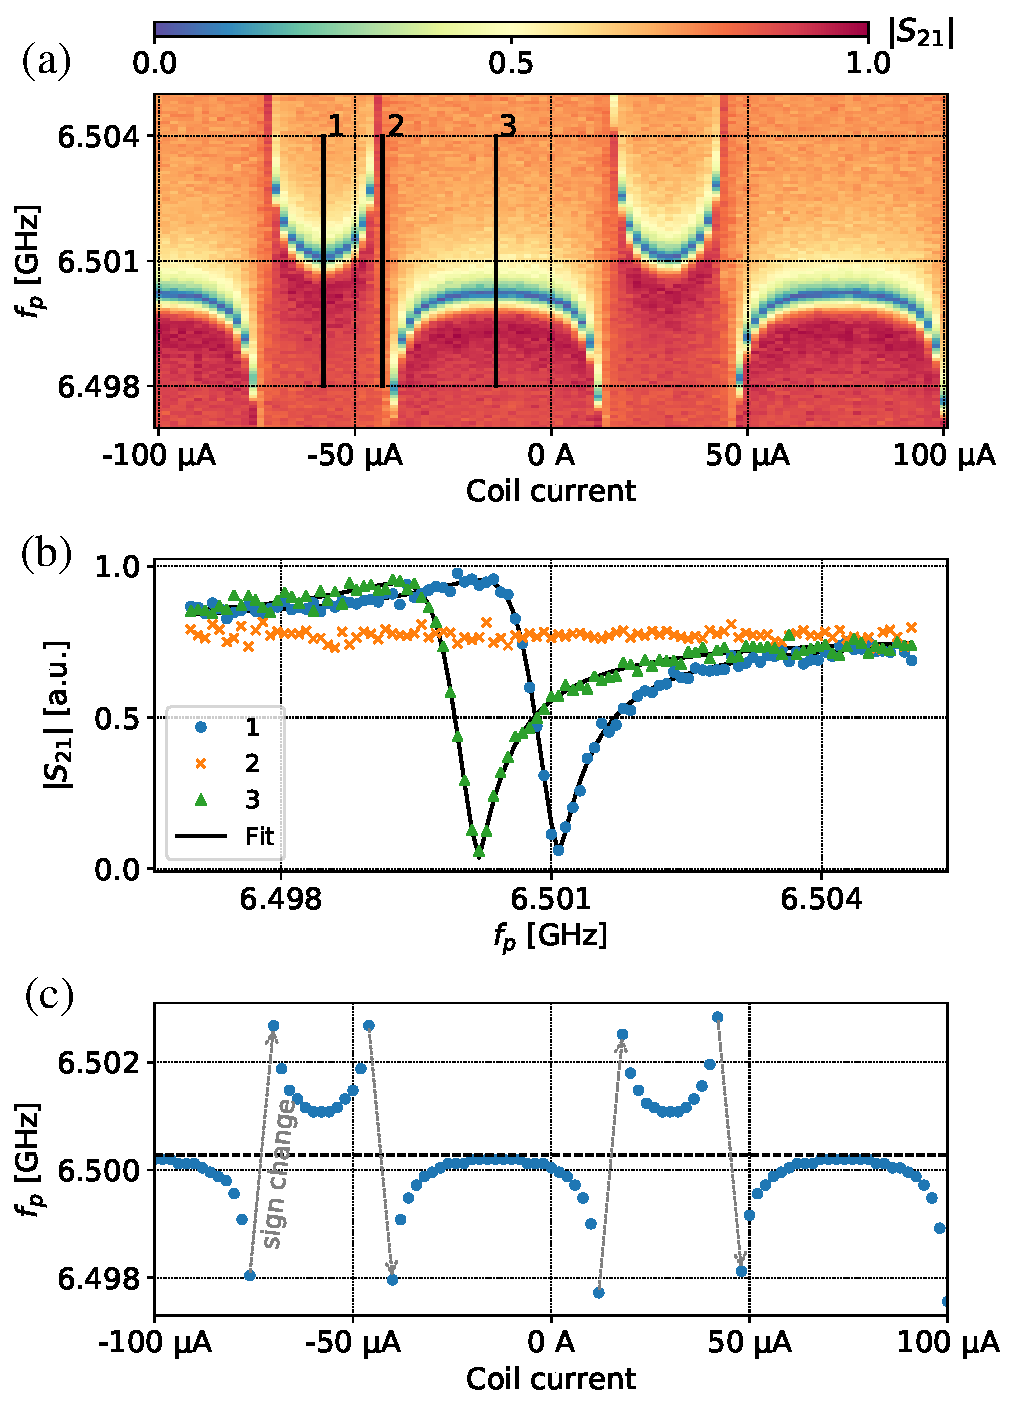
\includegraphics[width=\linewidth]{anti_subplots}
\caption{(a) Raw experimental heatmap of $|S_{21}|$ depending on the probe frequency $f_p$ and the coil current $I$. (b) Slices of the transmission from (a) showing two slices (1,3) with fits and a plateau 2 with no dip. (c) Extracted resonance frequency $f_r(I)$ (blue dots) and mean frequency value over all currents $\langle f_r \rangle_{I}$ (black dashed line). Grey arrows show where $f_r - \langle f_r \rangle_{I}$ changes sign.}
\label{fig:anti_exp}
\end{figure}

Now, knowing the internal structure of the data, we outline our algorithm to extract the Hamiltonian parameters from them. The main idea is to fit the model \eqref{eq:f_r} to the data in \autoref{fig:anti_exp}(a) in the sense of maximum likelihood estimation\cite{bishop2006} (MLE, see also Appendix \ref{sec:ML}). To reduce the complexity of the estimation in terms of the number of parameters, we first perform the MLE of the resonator frequency by fitting only along the $f_p$ axis using an external fitting library called \textit{circlefit}\cite{probst2015}. This removes the extra dimension from the data which now may be compared directly with the model leaving only 6 fitting parameters. Assuming normal distribution of noise in the estimated $f_r$, the MLE is equivalent to a non-linear least-squares problem with global optimization. It is a complex task, firstly, due to the periodic dependence of the frequencies on current $I$ and the unknown position of the qubit sweet spot $I_{ss}$ and, secondly, due to the strong non-linearity of \eqref{eq:f_r} and \eqref{eq:tr_spectrum} on other parameters. Fortunately, it is possible to get a good initial guess for $\Pi$ and $I_{ss}$ and then do a brute force search for the solution in other variables due to the well-defined bounds for each of them. Finally, we can polish the result in all six parameters using a local optimizer.

The detailed description of the method which uses \autoref{fig:anti_exp}(a) as an example is presented below. As it has already been mentioned, the chosen type of the resonator-qubit arrangement which yields the avoided crossings pattern is not unique; however, the other two cases are treated the same way.

\subsection{Extracting resonance frequency}\label{sec:extract_fr}

The resonator curve MLE is based on the \textit{circlefit} library which does the least-squares fitting of various types of microwave resonators. For each current $I$, it fits the complex transmission $S_{21}(f_p)$ which for a single resonator is a circle on the complex plane\cite{probst2015}. For brevity reasons, we do not present here the full complex fits; however, as an illustration in \autoref{fig:anti_exp}(b) one can see the absolute values of the optimized models (solid black lines) that match well with the absolute values of experimental data taken from slices 1 and 3 of \autoref{fig:anti_exp}(a). Finally, from the optimal model parameters we obtain the resonance frequency $f_r(I)$ depending on current. A possible caveat is that for some $I$ values the resonance dip may disappear (see \autoref{fig:anti_exp}(b), slice 2) so the resonator fit would fail. Therefore, such slices are excluded in advance via a threshold condition.

The resulting plot of the extracted resonator frequency versus current $I$ is shown in \autoref{fig:anti_exp}(c) (blue dots). There are some current values located between the branches where the data points are missing, as expected, due to the absence of the resonance. Additionally, we plot here the mean value of the detected frequencies shown as a dashed black line. This parameter is important since it, will firstly, serve as an initial guess for the cavity frequency of the model \eqref{eq:f_r}: $f_c \approx \langle f_r \rangle_{I}$ and, secondly, will be used in the period and phase extraction algorithm which tracks the changes of the sign of the value $\Delta f_r = f_r - \langle f_r \rangle_{I}$ (marked as grey dashed lines in \autoref{fig:anti_exp}(c)). Locating these sign changes allows to find the qubit sweet spot without fittig the full model.

\subsection{Extracting period and sweet spot locations}

As we have stated above, one of the obstacles for the fitting is the periodicity of the data on one of the fitting parameters. Along with the equally unknown phase of the signal, this leads to the presence of many local minima in the loss function which impede the progress of iterative optimization algorithms. In other words, the unknown parameters $\Pi$ and $I_{ss}$ are preventing us from finding the global minimum. So it would be very convenient to determine the period and the sweet spot location without fitting the full model \eqref{eq:f_r} to alleviate the stated problem. In the absence of noise, this would be a trivial task. Indeed, one would just need to find the sign changes in $ \Delta f_r $ directly by traversing the array of its values, and then compute the period as the distance between two same sign changes, and the sweet spot location as the point between the adjacent ones. However, in the conditions of experiment, the noise to some extent is always present, and it  so below we suggest a solution that is insensitive to local sporadic perturbations of the data.

\begin{figure}
	\centering
	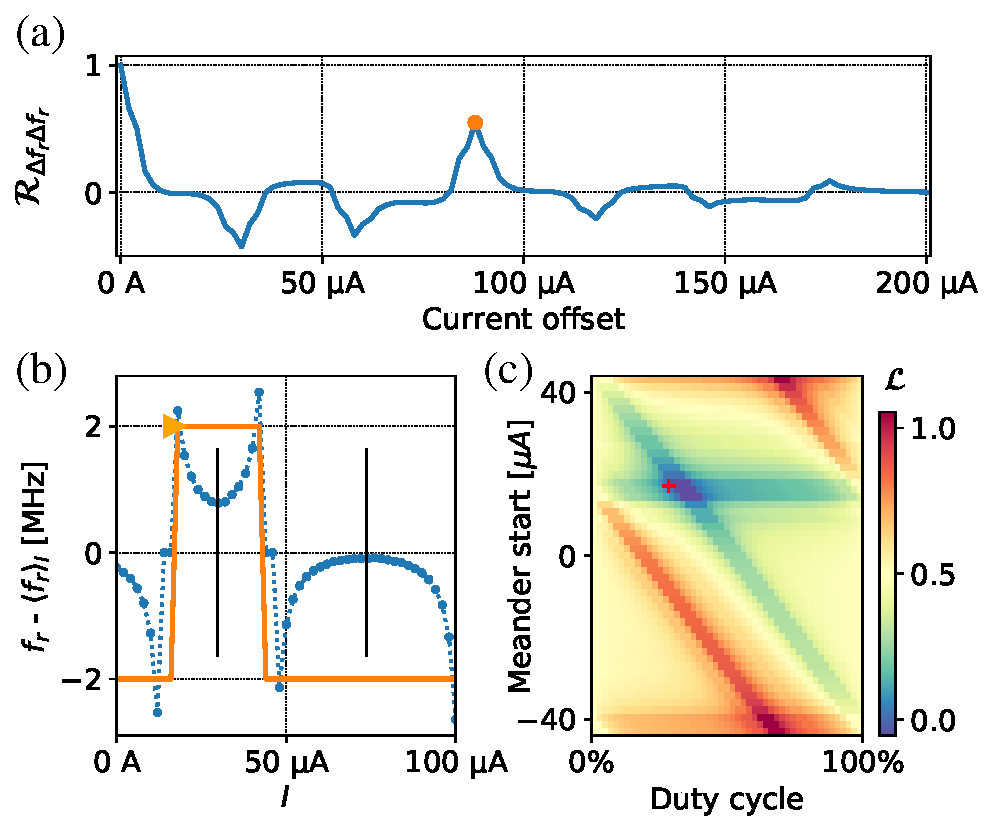
\includegraphics[width=\linewidth]{per+phase}
	\caption{Period and phase extraction procedure. (a) Autocorrelation function depending on the current offset $\Delta I$ shows a prominent local maximum at $88\ \mu$A (orange dot). (b) Construction for phase estimation; $\Delta f_r = f_r-\langle f_r \rangle_{I}$ (blue) is fitted with a square wave (orange, start marked with a triangle). Vertical bars mark candidate sweet spots. (c) Loss function (normalized) for the square wave fitting procedure from (b); red cross indicates the parameters of the meander shown there.}
	\label{fig:per+phase}
\end{figure}

An obvious method to find analytically the period and the phase (here, the phase is equivalent to $I_{ss}$) of a signal is the Fourier transform. Fast Fourier transform (FFT) should be applied to the data, and then the peak of the largest magnitude in the spectrum would give the likely frequency and the phase of the signal. FFT works well for the continuous curves, but it becomes inconvenient for the avoided crossings pattern due to the complexity of its spectrum caused by discontinuity. Moreover, FFT is not very accurate when the data contains only a couple of periods. A more robust tool to find the period in a given dataset $y$ especially when it contains just a few periods is the autocorrelation function $\mathcal{R}_{y y}(l) = \sum_n y_n y_{n-l}$. The location of the largest of its local maxima (except for $l=0$) equals exactly the sought period\cite{parthasarathy2006}. However, this is only true when the mean value of the function is zero; otherwise, $\mathcal{R}_{y y}(l)$ would be linear with a steep slope that may smear out all the extrema. Therefore, instead of directly calculating the autocorrelation of $f_r (I)$ we consider the standardized function $\Delta f_r (I)$ introduced above which has zero mean and the same period. For this function, the autocorrelation function $\mathcal{R}_{\Delta f_r \Delta f_r}(\Delta I)$ depending on the current offset $\Delta I$ is shown in \autoref{fig:per+phase}(a). As one can see, $\Delta I$ spans 200 $\mu$A just as the data itself. This means that to calculate $\mathcal{R}_{\Delta f_r \Delta f_r}(\Delta I)$ the data is being zero-padded at all $\Delta I$ except for $\Delta I = 0$, and this is why we get diminishing correlation peaks at $\Pi$, $2\Pi$, etc. The orange dot in the plot shows the highest local extremum of $\mathcal{R}_{\Delta f_r \Delta f_r}(\Delta I)$ at 88 $\mu$A. It is a very prominent peak and can be easily distinguished among all others. There is as well a small peak at 176 $\mu$A which corresponds to $\Delta I = 2\Pi$. Note that the the autocorrelation function is not ideally smooth and has some abrupt bends on the sides of the peaks. This happens because there were some missing points in the data (corresponding to the plateaus of \autoref{fig:anti_exp}(b)) that were replaced by zeros to ensure the \fxnote*{'more accurate' here is better than 'correct'}{correct} mapping between the current indices and current values. This zero padding may be noticed as well in \autoref{fig:per+phase}(b).

The problem with the autocorrelation function is that it does not tell us anything about the phase of the signal, i.e. the exact location of the sweet spot current. Therefore, after having found the period, we need another method to precisely determine $I_{ss}$. This method consists of finding the global maximum of the zero-lag correlation function $\mathcal{R}_{\Delta f_r S}(0)$ between $\Delta f_r(I)$ and a square wave $S(I, \Pi, \phi, D)$ having the same period but unknown phase $\phi$ and duty cycle $D$ which is the relation between the horizontal spans of the ``high'' and ``low'' levels of the wave. 
The values of the ``high'' and ``low'' levels must be opposite, i.e. 1 and -1, and the magnitude does not matter.  An illustration of a square wave function satisfying the optimal condition is presented in \autoref{fig:per+phase}(b) in orange. The phase $\phi$ (in $\mu$A) denotes the x-coordinate of the first point after the rising edge, and is marked with a triangle. Generally, the idea behind this is to robustly detect sign changes that were shown back in \autoref{fig:anti_exp}(c). Since $\mathcal{R}_{\Delta f_r S}(0) = \sum_I \Delta f_r(I) \cdot S(I) $, it gains value if $\Delta f_r$ and $S$ are of the same sign for a certain $I$. Therefore, the combination of $\phi, D$ that ensures the maximal number of points where $f_r(I)\cdot S(I)>0$ (the one that we are looking for) delivers the global maximum to $\mathcal{R}_{\Delta f_r S}(0)$. This approach will still work correctly even if the mean value $\langle f_r \rangle_{I}$ does not lie exactly between the branches in the avoided crossings pattern and intersects one of them since the period $\Pi$ is already found and is fixed. 

The optimal $\phi$ and $D$ are found using the brute force algorithm. It calculates the loss function $\mathcal{L} = - \mathcal{R}_{\Delta f_r S}(0)$ on a $50 \times 50$ grid of $(\phi, D)$ and takes the minimal value of all. This method is stable and universal due to the evident boundaries on $\phi \in [-\Pi/2,\Pi/2)$ and $D \in [0, 1]$. The loss function topography for the avoided crossing patterns is nicely structured and for our example is shown in \autoref{fig:per+phase}(c). One peculiarity is that instead of a single minimum it has an area of the same minimal value. Again, this effect comes from the missing zero-padded $f_r$ points at some $I$ values. However, any value from this valley suits well enough for our purposes, and the algorithm finds no difficulty in locating it.

Having found values for $\Pi,\ \phi$ and $D$ we now can finally calculate the current of the transmon sweet spot in the case of the avoided crossings pattern:
\begin{align*}
I_{ss} = 
 \phi + \Pi (1+D)/2.
\end{align*}
Alternatively, for the continuous patterns we need to apply a different formula:
\begin{equation*}
I_{ss} = \phi + \Pi D/2.
\end{equation*}
Since at this point the algorithm does not yet know which type of the pattern it observes, it may apply some heuristic to guess which equation to apply. When the noise is not too large, such heuristic may be to calculate the maximal absolute differential of the frequency data: $\max_{i>0} |f_{r,i} - f_{{r,i}-1}|$, and compare it to the peak-to-peak amplitude: $\max_{i,j} | f_{r,i} - f_{r, j}|$. For the avoided crossings these values are close and for the smooth dependencies they are not. However, in case of a strong noise this indicator may fail, and the program will have to check both current values to be $I_{ss}$ by fitting the full model two times, and then choose among the two possibilities based on the maximal likelihood.


\subsection{Full model fitting}


\begin{figure}
	\centering
	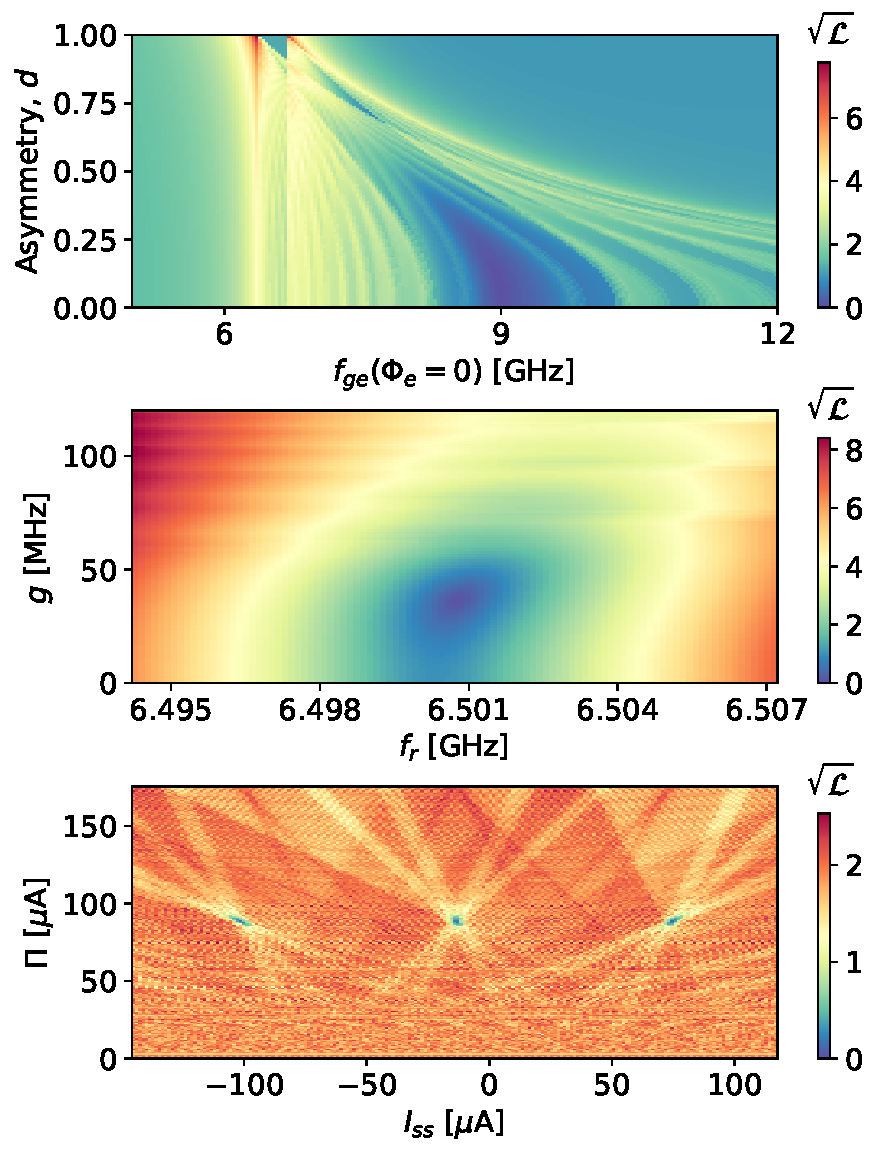
\includegraphics[width=\linewidth]{loss1}
	\caption{Slices of the loss function \eqref{eq:loss} for the full model and experimental data from the example made around the optimal point. Root-mean-square per-point loss $\sqrt{\mathcal{L}}$ is in MHz. (a) $f_{ge}^{max}$ and $d$ are varied, other parameters optimal. A large valley is located near 9 GHz, and some smaller locally minimal ones are present all around. (b) $g$ and $f_r$ are varied, others optimal. The loss function for these two parameters is well-conditioned near the optimum. (c) $\Pi$ and $I_{ss}$ varied, others optimal. This subplot illustrates a complex structure of local minima around the true one which we find analytically.}
	\label{fig:loss}
\end{figure}


Having performed the aforementioned preliminary steps, it is now possible to fit the full model to the extracted points. To do this, we employ brute force optimization combined with the Nelder-Mead simplex downhill algorithm\cite{nelder1965} to polish the brute force result. For both methods, we use a common loss function that is based on the maximum likelihood method (again, we presume Gaussian distribution of the points around the model). 
For the known probe frequency span of the data $\Delta f_p$ (\autoref{fig:anti_exp}(a), whole y-axis) and the set of $N$ extracted points $\{p_i\} = \{(I_i, f_{r,i})\}$, we calculate the loss function as
\begin{align}
\mathcal{L} &= \sum_{i=1}^N [f_{r,i} - \mathcal{M}(I_i,\ \Pi, \ I_{ss},\ f_c,\ g,\ f_{ge}^{max},\ d)]^2,\label{eq:loss}\\
\mathcal{M} &= \begin{cases}
f_+,\  |f_+ - f_c|< \Delta f_p/2 \\
f_-,\ \text{otherwise}, \label{eq:cond}
\end{cases}
\end{align}
where, as in the previous section, $$f_{\pm} = f_{\pm}(I_i,\ \Pi,\ I_{ss},\ \ f_c,\ g,\ f_{ge}^{max},\ d)$$
The condition of Eq. \eqref{eq:cond} means that we choose only the model frequencies that lie within the window $\Delta f_p$ around the model $f_c$ parameter. This ensures, firstly, that in the optimum we will not take any excess points outside the experimental frequency scan, and, secondly, that we have a singular model value for each current in case of avoided crossings.

To substantiate the choice of the optimization algorithms, we present in \autoref{fig:loss} three visualizations of the the defined loss function. The plots show how the function behaves if a certain pair of 6 model parameters is varied while others are optimal. From the plots it is obvious that the loss function is ill-defined and has a lot of local minima. Moreover, it may not be smooth everywhere because of the condition \eqref{eq:cond}. The $f^{max}_{ge}$ and $d$ parameters present significant difficulty in terms of false minima and low curvature as can be seen from \autoref{fig:loss}(a). In contrast, $f_c$ presents the least difficulty, as can be seen from \autoref{fig:loss}(b). The last plot \autoref{fig:loss}(c) shows a very complex structure of the loss function and narrow optimal valleys and serves as an illustration of why the period and phase extraction algorithm is important.

\begin{table}
	\centering
	\begin{ruledtabular}
		\begin{tabular}{lll} 
			Parameter & Value range & Steps \\ 
			\hline
			$f_c$ & $\langle f_r \rangle_{I} \pm 1$ MHz & 3\\ 
			$g$ & 20 - 40 MHz & 5\\
			$f_{ge}^{max}$ &  4 - 12 GHz & 80 \\
			$d$& 0 - 0.9 & 9
		\end{tabular} 
	\end{ruledtabular}
	\caption{Grid specifications for the brute force algorithm for STS detection.}
	\label{tab:grid}
\end{table}

The brute force algorithm acts on the grid specified in \autoref{tab:grid}. The ranges in the grid are based on the usual design parameters of the qubit samples in our database, and the number of steps is chosen so that the algorithm reliably finds the optimal valley. After the coarse brute force optimization is done and the optimal valley is located, we apply the Nelder-Mead search on all 6 parameters.


\section{Results}

\begin{table*}
	\centering
	\begin{ruledtabular}
		\renewcommand{\arraystretch}{1.2}

		\begin{tabular}{*{13}{l}} 
			\multirow{2}{*}{\textbf{Parameter}} & 
			\multicolumn{4}{l}{\textbf{(a)}} & 
			\multicolumn{4}{l}{\textbf{(b)}} & \multicolumn{4}{l}{\textbf{(c)}}\\
			& Brute & N-M & $\sigma,\ \mathbb{H}^{-1}$ & Correct  & Brute & N-M & $\sigma,\ \mathbb{H}^{-1}$ & Correct  & Brute& N-M & $\sigma,\ \mathbb{H}^{-1}$ & Correct  \\
			\hline
			$f_c$, GHz &6.5003 & 6.5007 &  4$\times 10^{-6}$ & n/a & 6.962 & 6.9631 & 1.6 $\times 10^{-4}$  & n/a &  6.47 & 6.465& 2$\times 10^{-4}$ & n/a\\ 
			$g$, MHz & 24 & 35.8 & 0.17 & n/a & 36 & 64.9 & 15 & n/a & 36 & 86.1& 1 &n/a\\
			$f_{ge}^{max}$, GHz & 8 &\textbf{8.97} & 0.013 & \textbf{9.04} &10.3& \textbf{11.3}& 1.35 & \textbf{9.08}& 6.3& \textbf{5.89}&0.01&\textbf{5.9}\\
			$d$ &0.5& \textbf{0.09}& 0.013& \textbf{0.13} &0.5&\textbf{0.49} &0.07&\textbf{0.6}&0.1& \textbf{0.25} & 0.05 &\textbf{0.3} \\\hline
			Loss, kHz & 251 & 20 && &338& 51 & & &2038& 149&&
		\end{tabular} 
	\end{ruledtabular}
	\caption{Analysis of optimal parameters found for the three cases in \autoref{fig:anti_fit_cases} after the brute and Nelder-Mead (N-M) optimizations. $\sigma, \mathbb{H}^{-1}$ columns stand for \fxnote*{Standard deviation should be probably replace by variance $\sigma^2$, and, more precisely, by 'lower bound of variance' }{the estimates for the standard deviations} found from the diagonal of the \fxnote*{Does covariance matrix here actually mean Fisher information matrix?}{covariance matrix which was calculated using the Hessian} $\mathbb{H}$ of the loss function at the optimum.\fxerror{Replace column name 'Correct' with 'TTS' or similar and to separate TTS from the rest by vertical line or somehow. Otherwise this column gives an impression that method does not work properly - N-M is sometimes very very far from 'Correct'!}}
	\label{tab:sts_results}
\end{table*}

\begin{figure*}
	\centering
	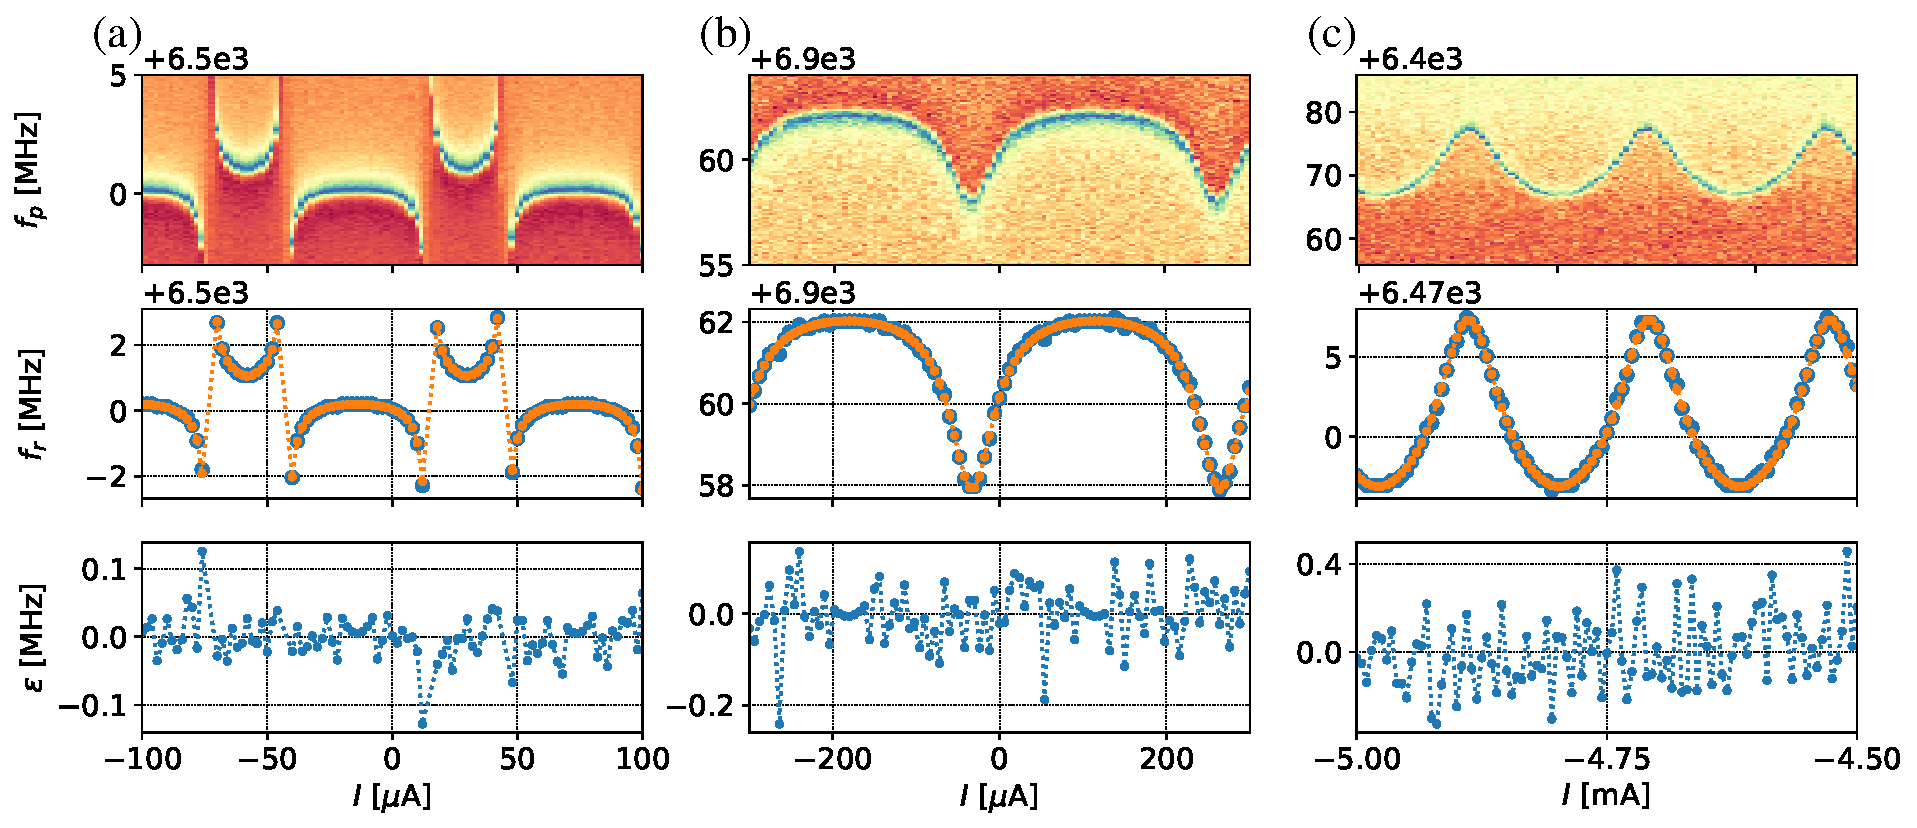
\includegraphics[width=\linewidth]{fit_cases}
	\caption{The results of the algorithm execution on three experimental examples from our database. In the upper row, original images are presented. In the middle row, the data  (blue dots) and the fitted model (orange connected dots) are shown. In the lower row are errors $\varepsilon$. (a) Avoided crossings pattern; per-point RMS error around 30 kHz. (b) The qubit entirely above the resonator; per-point RMS error around 60 kHz. (c) The qubit below the resonator; per-point RMS error around 150 kHz.\fxnote{Since $f_r$ differs by order of magnitude in cases (a) vs (b) and (c), showing RMS in kHz may be considered misleading. May be MAPE is better in this case? }}
	\label{fig:anti_fit_cases}
\end{figure*}

The algorithm was implemented in Python using  routines of the SciPy\cite{scipy} library. We present here examples of the detection for all possible qubit-resonator dispositions.  The resulting fits are presented in \autoref{fig:anti_fit_cases} along with the original data and the error plots characterizing the quality of fit quantitatively; we will further reference them as (a), (b) and (c) respectively.

\subsection{Fit quality analysis} 

In \autoref{tab:sts_results} we analyse the fitting resuls for the three cases. Comparing the brute estimation and the final result after the Nelder-Mead search, one can see that the chosen algorithm order works as expected: the exhaustive search finds good initial conditions for the Nelder-Mead, and there is a significant improvement in the loss value of the polished result compared to the brute estimation which is due to the more accurate determination of the cavity frequency $f_c$ which leads as well to major shifts in optimal $g$, $f_{ge}^{max}$ and $d$.

However, in turns out that the optimal qubit parameters and coupling strength may be relatively inaccurate. For example, in case (b) for $f_{ge}^{max}$ we see a more than 2 GHz difference between the optimal and the \fxerror*{Replace 'correct' with 'more accurate' here. I believe TTS does not give the 'correct' value, so it is an error here}{correct} value found for the sample with TTS. For (a) and (c), the differences in $f_{ge}^{max}$ are much smaller (about 10-70 MHz) but instead we see errors in $d$ (around 10\%). Inaccuracy in the qubit parameters may be qualitatively explained by the low sensitivity of the resonator frequency to the qubit frequency when they are far away and by the strong correlations between the parameters. Concerning $f_c$ and $g$, it is not possible to extract the true values for them independently, so we leave the corresponding entries empty.

To quantify the errors in the fit parameters, we have calculated numerically the Hessians $\mathbb{H}$ with respect to all fitting parameters at the optimal point for the three cases using the \textit{numdifftools}\cite{numdifftools} package (see Appendix \ref{sec:ML} for details). In \autoref{tab:sts_results}, columns $\sigma, \mathbb{H}^{-1}$ we show the square roots of diagonal of the resulting variance-covariance matrix that estimate the standard deviations in the fit parameters. As can be seen, in case (b) estimated variances for $g$ and $f_{ge}^{max}$ are much higher than ones for the cases (a) and (b), explaining the larger errors. Additionally, using the principal component analysis of the Hessians, we find that the most unconstrained component eigenvector contains the correlated parameters $f_c,\ g,\ f_{ge}^{max},\ d$, and the second one (being an order of magnitude smaller) consists of $\Pi$ and $I_{ss}$. To reduce the correlations, one may chose another parametrization of the model, i.e. replace $d$ and $f_{ge}^{max}$ by $ E_{JJ}^{max} $ and $ E_{JJ}^{min} $. However, the accuracy of the fit using the presented parametrization is enough for practical applications.

\begin{figure*}
	\centering
	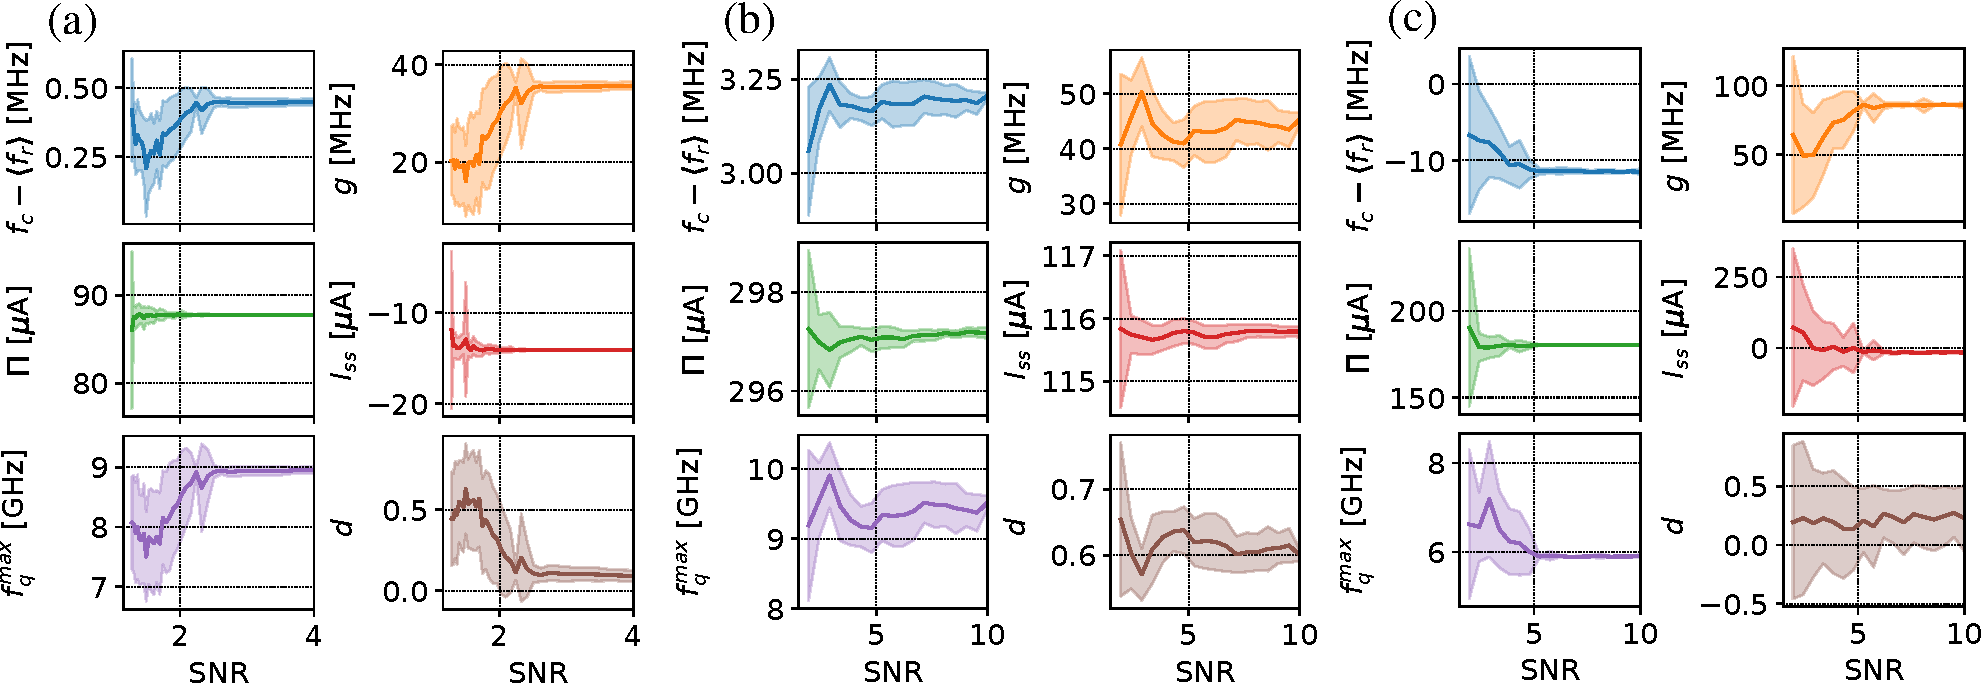
\includegraphics[width=\linewidth]{noise_test}
	\caption{Behaviour of the algorithm on the real data from \autoref{fig:anti_fit_cases} with added gaussian noise of varying power (i.e., with artificially reduced SNR). The clouds show the 25th and 75th percentiles of the optimal parameter samples for 50 realizations of the added noise, solid lines show median values. (a) Original data SNR is 19. The algorithm is accurate above SNR=2.5 (well below the original SNR), but is still robust down to SNR=1.3. (b) Original data SNR is 4.7. The qubit frequency and asymmetry are not determined accurately, but the algorithm is stable above SNR=1.5. (c) Original data SNR is 3.14. The algorithm is robust above SNR=1.75, and is only uncertain in determining the asymmetry $d$.}
	\label{fig:noise_test}
\end{figure*}

\subsection{Testing noise robustness}

To stress test the algorithm, we artificially deteriorate the data from \autoref{fig:anti_fit_cases} by adding complex Gaussian noise of various variances to the complex data at each ($f_p$, $I$) before fitting. However, since the original data already contains noise, and its variance $\sigma_0$ may differ for different \fxnote*{Replace 'measurements' with 'experiments'? }{measurements}, we first have to define a common scale for all three cases (a), (b) and (c) to be able to compare them. The signal-to-noise ratio (SNR) turns out to be a sensible universal measure of noise, and is defined for our data in a similar manner to the SNR in the resonator fitting tests\cite{probst2015}. Since the data for a resonator lie on a circle in the complex plane, it is convenient to take its radius $r$ as the signal amplitude. Then, if the total noise is of the form $\frac{\xi_1+i\xi_2}{\sqrt 2}$, where $\xi_1,\ \xi_2$ distributed normally with zero mean and variance $\sigma$, the SNR is defined as 
\begin{equation}
r/\sigma = r/(\sigma_0+\sigma_1),
\label{eq:SNR}
\end{equation}
where $\sigma_1$ is the added noise. Obviously, the resulting SNR in this scale can't be larger then the original SNR=$r/\sigma_0$. 

Using the described common scale for the measurements (a), (b) and (c), we test the algorithm stability by launching it 50 times for different added noise realizations for a range of variances $\sigma_1$: the added noise power is steadily increased, and the resulting SNR is being calculated with \eqref{eq:SNR}. We then record all fitting results, and calculate their mean value, 25\textsuperscript{th} and 75\textsuperscript{th} percentiles for each variance $\sigma_1$.  Since the original noise is fixed, the variance of the fitting results will go to zero at SNR=$ r/\sigma_0 $ where the added noise is negligible and the fit converges to the same values as in \autoref{tab:sts_results}. 

In \autoref{fig:noise_test} we plot the results of the test outlined above. As one can see from the graph, the algorithm becomes stable above SNR=3, and the lowest SNRs before divergence occurs are around 2. The original data SNR for (a) is 19, and thus in the tests $\sigma_1 > 5\sigma_0$. Conversely, the original data SNR for (b) and (c) are much lower, and thus $\sigma_1 \approx \sigma_0$ in the tests. This means that for (b) and (c) the variance of the fitting results shown with the clouds in \autoref{fig:noise_test} is lower than it would be if all the noise was generated. To cope with this problem, in Appendix \ref{sec:ML} we test the algorithm on the synthetic data where the noise may be fully controlled.

In overall, the detection algorithm is stable even at very low SNRs where the patterns are barely visible by the human eye. The performance is limited mostly by the resonator frequency detection part.


\subsection{Performance}


\begin{table}[b]
	\begin{ruledtabular}
		\begin{tabular}{llllll}
			&Extract $f_r$& $\Pi$, $I_{ss}$ & Brute &N-M &
			\textbf{Total}\\\hline
			\textbf{Time}, s& 2.72& 0.3&2.79&1.37&7.34\\
			\textbf{Ratio}, \% & 37 &4 &38 &18 &100
		\end{tabular}
	\end{ruledtabular}
	\caption{Performance of the algorithm on a 2.5 GHz 2-core i5-5337U CPU for the case (a). Most of the time is taken by the the $f_r$ extraction and the brute search steps.}
	\label{tab:performance}
\end{table}

We have tested the performance of the algorithm on a 5-year old 2-core Intel i5-3337U CPU @ 2.5 GHz. The results are presented in \autoref{tab:performance} for the case (a).  As can be seen, the procedure takes around 7 seconds to complete. On a contemporary Intel Core i7-7700 CPU, it takes about two seconds. 

The heaviest parts are the frequency extraction part with the $circlefit$ library (2.7 seconds, most time spent in iterative calibration fits) and then brute search and Nelder-Mead optimization where the time costs mostly come from the square root calculation necessary for Eqs. \eqref{eq:tr_levels} and \eqref{eq:branches2}. However, this is still fast, firstly, because recording a resonator spectrum such as one in the example takes around 20 seconds, and, secondly, it is much faster than doing it manually. 

Basing on the complexity of calculating the value of the loss functions, the frequency extraction scales at least as $\mathcal{O}(NM)$ if $N$ and $M$ are the number of points for $I$ and $f_p$, respectively, and the following optimization scales linearly with $N$. 


\section{Discussion}


In summary, we have developed and implemented a method for automatic processing of single-tone spectroscopic data that uses maximum likelihood estimation to extract the physical parameters of cQED systems from a measurement result. We have shown that it is possible to estimate all of the system parameters by observing only the behaviour of the resonance peak for any type of the qubit-resonator disposition. Our method is robust to strong noise down to SNR=3 and is fast enough to be used in practice. Despite the fact that the accuracy of the algorithm does not allow to start gate calibrations right after the single-tone spectroscopy step, it is enough to perform two-tone spectroscopy with significantly reduced scan ranges to reduce time costs. Additionally, basing on the fit quality it is possible to distinguish between functional and defective samples.

The software implementation of the algorithm in Python may be found on GitHub\footnote{\url{https://github.com/vdrhtc/Measurement-automation/blob/master/lib2/fulaut/AnticrossingOracle.py}}. The code as well accepts data as a Python dictionary with corresponding keys. Currently, only transmon qubits are supported; however, we are ready to implement another type of qubit if needed.

\begin{figure}[b]
	\centering
	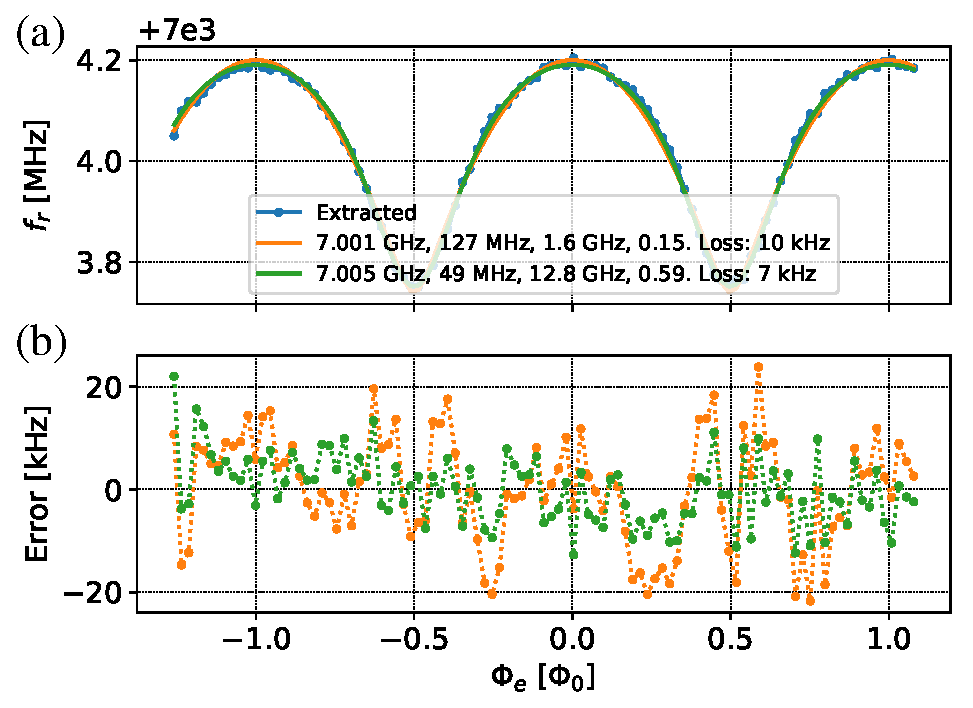
\includegraphics[width=\linewidth]{alternative_fits}
	\caption{(a) Two alternative fits (orange and green lines) for the same data (blue dots). The corresponding parameters $f_c,\ g,\ f_{ge}^{max}, d$ for the two alternative fits are in shown the legend along with the loss values. (b) Residuals for the two fits, in orange (qubit below) and green (qubit above the resonator).}
	\label{fig:alternative-fits}
\end{figure}


Considering the downsides of the suggested approach, we note that the implementation of the algorithm is not perfectly optimized: the brute force search is not fully parallel and may be replaced with a more sophisticated global optimization algorithm such as simulated annealing or basin hopping. Another problem that may slow down the execution is that for large qubit-cavity detunings and high noise two very different sets of parameters may minimize the loss function equally well. An illustration for this statement can be seen in \autoref{fig:alternative-fits}(a),(b) where the algorithm was launched twice using different grid ranges for $f_q^{max}$. In one case (orange) the search was done below, and in the other (green) above the mean resonance frequency $\langle f_c\rangle_{I}$. The resulting fits are almost equally accurate, and without other information about the system it is not be possible to reliably choose between the two. Therefore, some hints should be passed to the algorithm to avoid ambiguity; for instance, a prior probability density may be imposed on the parameter values and the MLE replaced with maximum a posteriori method. Otherwise, it would be necessary to check both possibilities with other methods, i.e. via two-tone spectroscopy. Since for the transmon qubits the case in \autoref{fig:alternative-fits} is the only type of ambiguity that may occur, we introduce an optional flag for the program that specifies where to look for the qubit during the brute force search: above or below the resonator.

Finally, in the future we are planning to use the proposed algorithm along with automatic two-tone spectroscopic measurements to build a full system that will automatically calibrate the qubit samples from scratch.


\section{Aknowledgements}


\appendix



\section{Transmon Hamiltonian}\label{sec:transmon}

\begin{figure}[b]
	\centering
	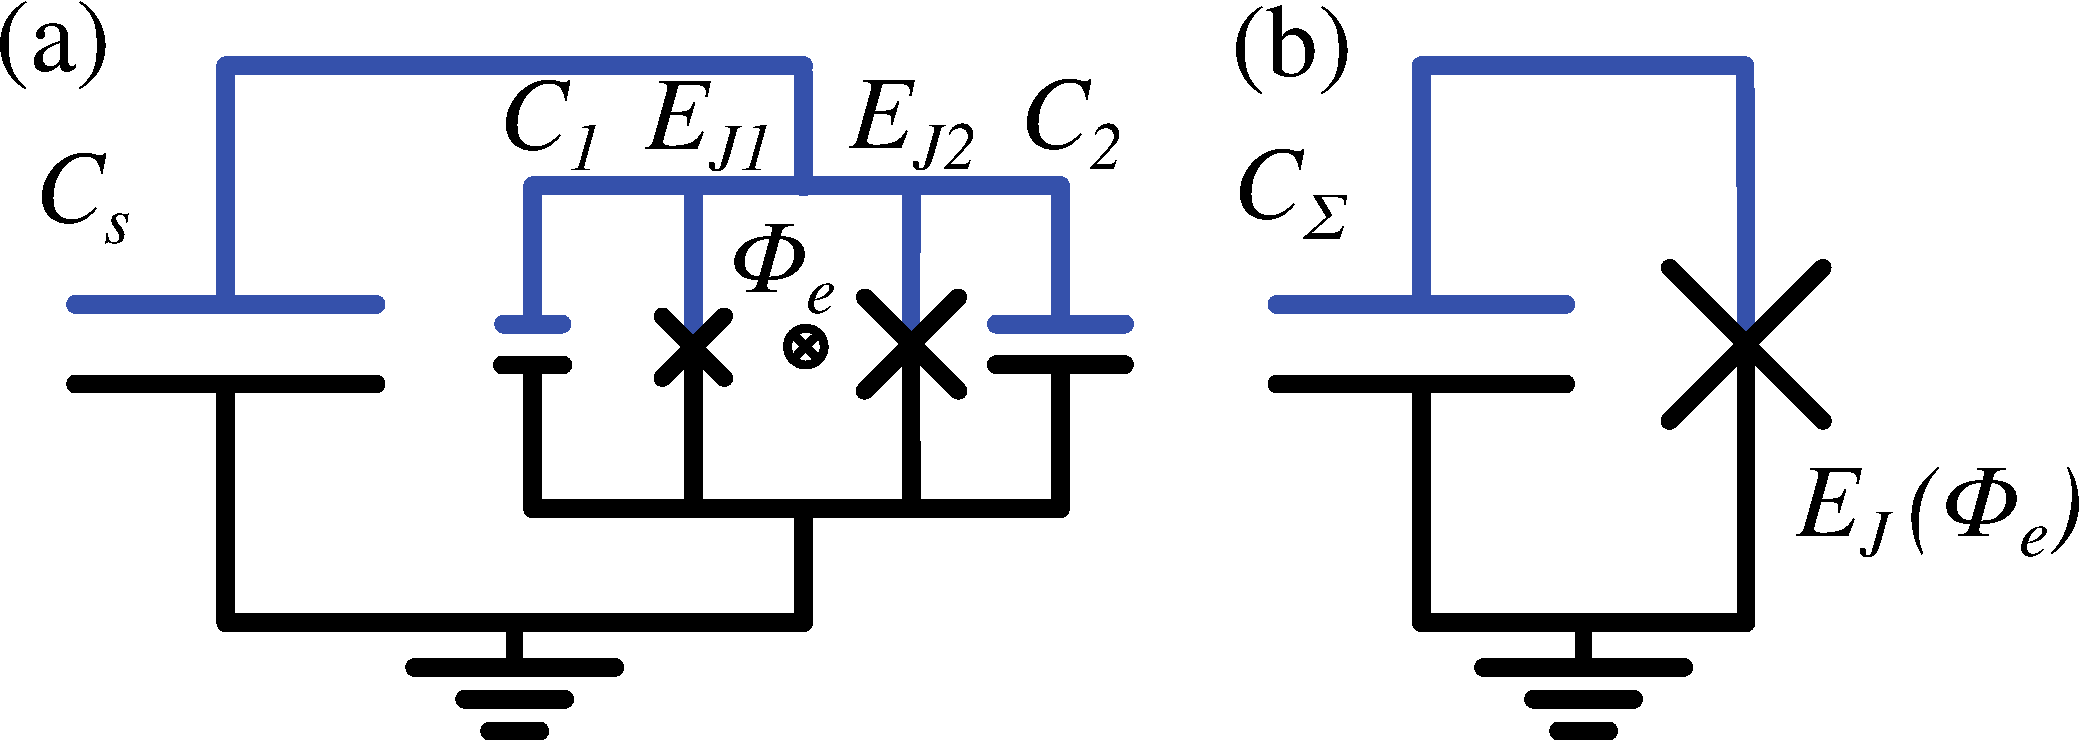
\includegraphics[width=\linewidth]{transmon}
	\caption{(a) A tunable transmon circuit with an asymmetric SQUID, $E_{J1} \neq E_{J2}$. (b) Equivalent transmon with tunable energy $E_{J}(\Phi_e)$ and unified capacitance $C_{\Sigma}$. The qubit island containing its single degrees of freedom is in blue.}
	\label{fig:trans}
\end{figure}

\begin{figure*}
	\centering
	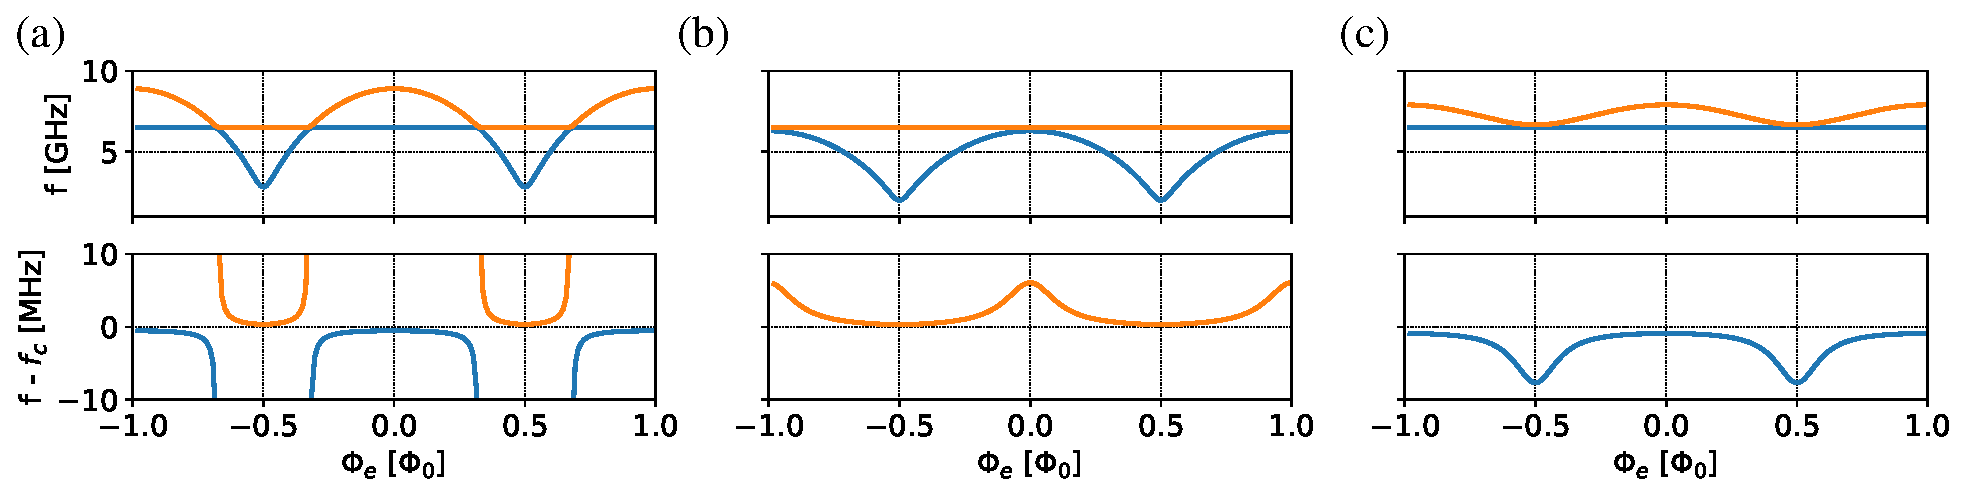
\includegraphics[width=\textwidth]{anti_theor}
	\caption{Frequency spectrum of the transmon-resonator system. Parameters used: $f_{ge}(0) \approx \sqrt{8E_C E_J(0)}/2\pi = 8.5$ GHz, $d=0.3$, $f_r=6.4$ GHz, $g = 30$ MHz. For each subplot two transition branches  $f_{\pm} = (E_{\pm,0} - E_{g,0})/2\pi$ are shown (orange and blue, respectively) both forming the resonator and qubit lines. As one can notice, there are three qualitatively different cases of the resonator-qubit disposition. Lower row shows a zoomed area around $f_c$ that looks differently in each case.}
	\label{fig:anti_theor}
\end{figure*}

The simplest version of this qubit consists of a Josephson junction shunted with a large capacitor. Flux tunability of the frequency is attained by replacing a single Josephson junction with a SQUID as in \autoref{fig:trans}(a) and applying external magnetic flux $\Phi_e$ to its loop. This scheme can be equivalently represented by a capacitively shunted junction of tunable Josephson energy, \autoref{fig:trans}(b). The Hamiltonian for such system is as follows: 
\begin{equation}
\hat{H}_{tr} = 4E_C \hat n^2 - E_J(\Phi_e) \cos \hat\varphi,
\label{eq:tr_ham}
\end{equation}
where $E_C = e^2/2C_{\Sigma}$, $C_{\Sigma} = C_s + C_1 +C_2$, is the charging energy, $\hat n$ and $\hat \varphi$ are the operators for the Cooper pair number and the phase of the qubit island. For the equivalent Josephson energy $E_{J}(\Phi_e)$ one obtains
\begin{equation}
E_{J}(\Phi_e) = E_{J\Sigma}\cos\left(\pi \Phi_e/\Phi_0\right) \sqrt{1+d^2 \tan^2 \left(\pi \Phi_e/\Phi_0\right)},
\label{eq:EJ_Phie}
\end{equation}  
where $E_{J\Sigma} = E_{J1}+E_{J2}$ ($E_{J1},\ E_{J2}$ are the single junction energies), $d = \frac{E_{J1}-E_{J2}}{E_{J1}+E_{J2}}$ is the asymmetry of the SQUID. As one can notice, the dependence is periodic in $\Phi_e$.

It is also possible to derive analytical expressions for the energy levels and transition frequencies for this type of qubits. The energy of the $m$\textsuperscript{th} level is (in the limit of $E_J\gg E_C$) \cite{koch2007}
\begin{equation}
E_m = m \sqrt{8E_J(\Phi_e) E_C} -\frac{E_C}{12}(6m^2+6m).
\label{eq:tr_levels}
\end{equation}
From this equation, the qubit transition frequency ($ \ket{0}\rightarrow \ket{1}$, or $ \ket{g}\rightarrow \ket{e}$, or the $ge$ transition) may be approximated as 
\begin{equation}
\begin{aligned}
f_{ge}(\Phi_e) &\approx \sqrt{8 E_J (\Phi_e) E_C} \\
&= f_{ge}^{max} \sqrt{\cos\left(\pi \Phi_e/\Phi_0\right) \sqrt{1+d^2 \tan^2 \left(\pi \Phi_e/\Phi_0\right)}},
\end{aligned}
\label{eq:tr_model}
\end{equation}
where $f_{ge}^{max} = \sqrt{8 E_J(0) E_C}-E_C$ is the maximal possible frequency. The approximation here is $E_C \approx E_C/\sqrt{\cos\left(\dots\right) \sqrt{1+d^2 \tan^2 \left(\dots\right)}}$  which gives significant errors only when $E_J\approx E_C$ (when $d$ is small and $\Phi_e\approx\pi/2$) and when the expression \eqref{eq:tr_levels} which itself is no longer valid. On the contrary, this approximation simplifies the model since now it depends just on two parameters ($f_{ge}^{max}, d$) instead of three. Therefore, we choose \eqref{eq:tr_model} as the theoretical curve in fitting.

One final note is that in the real-life applications is not possible to know directly the flux $\Phi_e$ that is threaded through the SQUID. The experimenter usually knows only the current $I$ (or voltage) which he applies to some coil that is connected inductively to the SQUID. Then $\Phi_e = M I + \Phi_r$, where $M$ stands for the mutual inductance of the coil and the SQUID, and $\Phi_r$ is some residual flux inherent to the sample. So, in the main text we only use the current $I$, the period in current $\Pi = \Phi_0/M$ and the sweet spot current $I_{ss} = -\Phi_r/M$ and not the corresponding magnetic fluxes.

\section{Circuit QED}\label{sec:cqed}

The readout of the superconducting qubits is now predominantly done using an ancilla system which is usually implemented as a superconducting microwave resonator which acts as an electromagnetic cavity in the standard cavity quantum electrodynamics (QED). Truncating the qubit to two levels ($ge$ transition), one may obtain the following Hamiltonian for the compound cavity-qubit system (in RWA):
\begin{equation}
\hat H/h = \frac{f_{ge}}{2} \hat \sigma_z + f_c \hat a^\dagger \hat a + g(\hat \sigma^- \hat a^\dagger + \hat \sigma^+ \hat a),
\end{equation}
where $f_{ge}$ is the qubit frequency, $f_c$ is the cavity frequency and $g$ is the coupling strength. As long as the RWA is done, this Hamiltonian may be diagonalized analytically\cite{blais2004}:
\begin{align}
E_{g, 0}/h &= \frac{f_c - f_{ge}}{2},\label{eq:branches1}
\\
E_{\pm, n}/h &= (n+1)f_c \pm \frac{1}{2}\sqrt{4g^2(n+1)+(f_{ge}-f_c)^2}.
\label{eq:branches2}
\end{align}

This is very convenient for our purposes. By substituting the dependence of the qubit frequency $f_{ge} \equiv f_{ge}(\Phi_e)$ into these equations, we can get straightforwardly the full system spectrum in dependence on the magnetic flux. In \autoref{fig:anti_theor} we have used the equations \eqref{eq:tr_model}, \eqref{eq:branches1} and \eqref{eq:branches2} to model a tunable transmon interacting with a cavity for various $\Phi_e$ and various $f_{ge}^{max},\ d$. In the lower row of the figure, one can see that it is possible to extract the dependence of the \textit{modified} cavity frequency $f_c^\prime$ on $\Phi_e$ (in the main text, we call it $f_r$ as the experimentally observed resonator frequency); for example, the avoided crossings pattern can be directly observed in \autoref{fig:anti_theor}(a), and the other two possible behaviours for the qubit entirely above or below the resonator in \autoref{fig:anti_theor}(b),(c). To shorten the notation, in the following we will define the corresponding branch frequencies of \eqref{eq:branches2} as $f_{\pm} = ( E_{\pm,0}-E_{g,0})/2\pi$.

\section{Maximum likelihood, Fisher information, Monte-Carlo testing}\label{sec:ML}

\begin{figure*}
	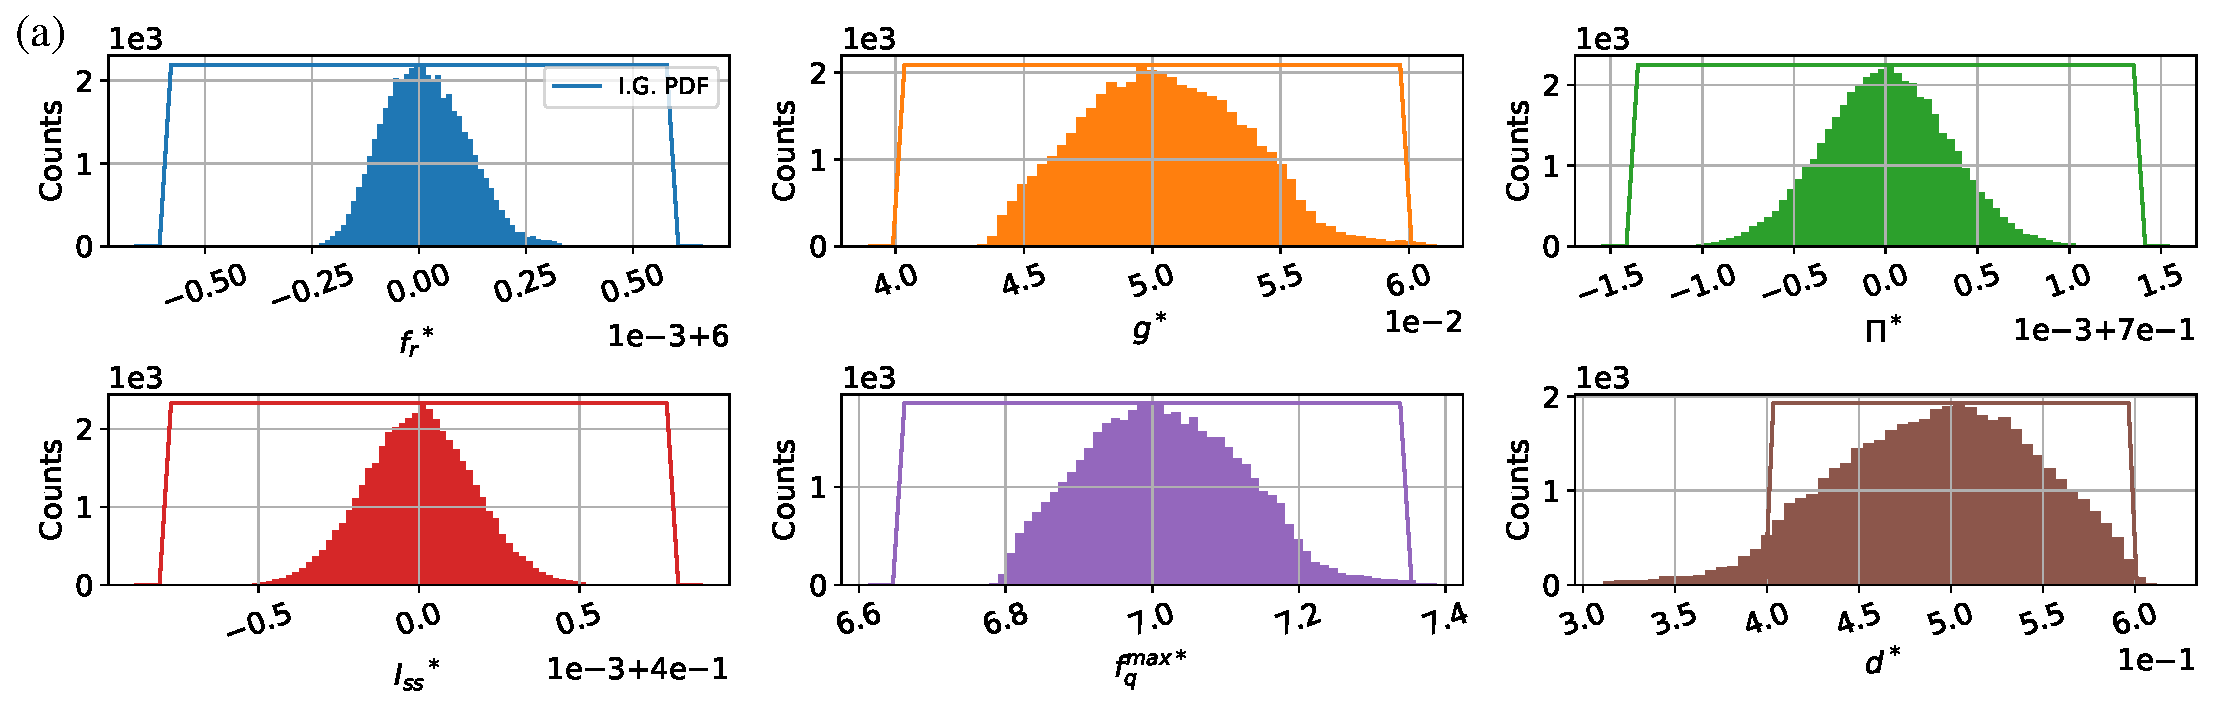
\includegraphics[width=\linewidth]{MC-test-tr}
	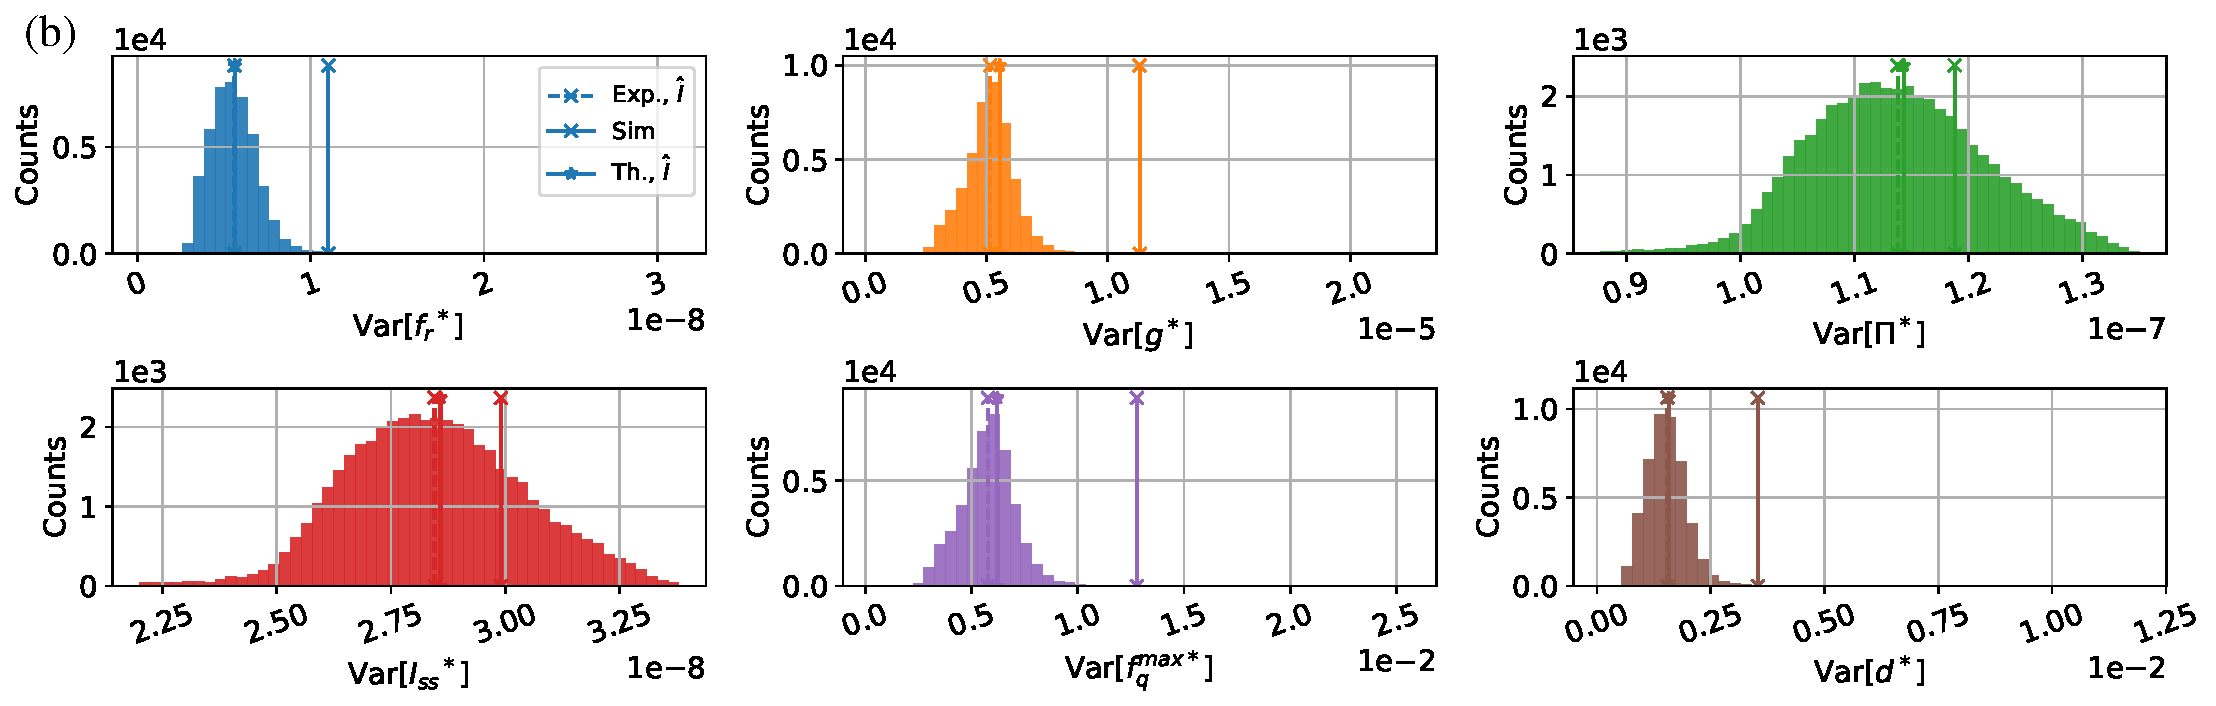
\includegraphics[width=\linewidth]{MC-test-tr-H}
	\caption{Monte-Carlo testing of the Nelder-Mead optimization step on the synthetic data (avoided crossings pattern). Model parameters $\mathbf{w}^0$ = ($f_r,\ g,\ \Pi,\ I_{ss},\ f_q^{max},\ d)^T$ were (6 GHz, 50 MHz, 0.7 mA, 0.4 mA, 7 GHz, 0.5)$^T$; the current $I$ took 1000 points between 0 and 1 mA. Added noise $\varepsilon$ was normal with $\sigma=1$ MHz. Fitting was run 5$\cdot 10^4$ times each with random initial points and a new noise realization. \textbf{(a)} Histograms of the estimator values for each fitting parameter. Solid lines show the probability density functions (PDFs) from which the initial guesses for the fits were drawn. \textbf{(b)} Analysis of the variance predicted by the Hessian. Histograms show the distribution of the variance lower bounds of the estimators calculated from 5$\cdot 10^4$ Hessians. Dashed lines with crosses show the expectation values of the histograms. Solid lines with star marks show the calculation with \eqref{eq:fisher_analytic}. Finally, solid lines with crosses show the experimental variances extracted from (a).}
	\label{fig:mc-test}
\end{figure*}

	
For a vector $\mathbf{w}$ of parameters, it is easy to calculate the likelihood $ \mathcal{L}(\mathbf{p}|\mathbf{w}) $ to observe the sample data points $\mathbf{p} = \{I_i, f_{r,i}\}_{i=0}^N$ if they are presumed to be normally distributed around the model ($\mathbb{N}_{\mu_i, \sigma}$, $\mu_i = \mathcal{M}(I_i, \mathbf{w}),\ \sigma = \text{const}$) and uncorrelated. The sought value is the product of the probability densities of individual data points:
\begin{equation}
\mathcal{L}(\mathbf{p}|\mathbf{w}) = \prod_{i=0}^{N} \frac{1}{\sqrt{2\pi}\sigma} \exp[ -(f_{r,i} - \mu_i)^2 / 2 \sigma^2]\label{eq:MLE} 
\end{equation}
The maximum likelihood method consists of finding the optimal parameter vector $\mathbf{w}^*$ such that $ \mathcal{L}(\mathbf{p}|\mathbf{w}^*) $ is the highest among all allowed $\mathbf{w} $. The vector $\mathbf{w}^*$ is called an estimator for the true parameter vector $\mathbf{w}^0$. If we take the negative logarithm of the likelihood, we will get the negative log-likelihood function:
\begin{align*}
- \ln \mathcal{L}(\mathbf{p}|\mathbf{w}) &= \sum_{i=0}^N (f_{r,i} - \mu_i)^2 / 2 \sigma^2 + N \ln\sqrt{2\pi}\sigma.
\label{eq:logL} \\
&= \chi^2/2 + N\ln \sqrt(2\pi)\sigma
\end{align*}
Minimizing this function is equivalent to maximizing the likelihood since the logarithm is monotonic. As the second term in the right part does not depend on $\mathbf{w}$, the task is reduced to minimizing the sum of squares, or the $\chi^2$; this argument dictates the chosen form of the loss function \eqref{eq:loss}. 

Next, we consider \fxnote*{Actually, we are trying to find the lower bound of our estimator's variance, not error of the fit}{the error of the fit}. \fxerror*{Unfortunately, we can't presume than our estimator is an unbiased one. It has to be proved! Otherwise, Cramer-Rao includes the estimator's bias into the estimated variance.]}{Presuming that $\mathbf{w}^*$ is an unbiased estimator of the true parameter vector}, we can use the multivariate Cramér-Rao inequality to bound its variance from below. In the general case, the inequality is as follows:
\begin{equation}
\text{Var}_\mathbf{w}[\mathbf{w}^*] \geq \text{diag} [\hat I(\mathbf{w})^{-1}],\ \forall\,\mathbf{w}.
\label{eq:cramer-rao}
\end{equation} 
Here $\text{Var}_\mathbf{w}$ means the variance of the estimator when the \emph{true} model distribution parameters are $\mathbf{w}$, and $ \hat I(\mathbf{w}) $ is the Fisher information matrix.Since \fxwarning*{We can't say in general whether Fisher information depends on $\mathbf{w}$ or not. Keener gives the example 4.10 where it does depend and 4.11 where it does not} {this matrix depends on $\mathbf{w}$}, \fxerror*{If Fisher information does depend on true $\mathbf{w}$, we can't say that its evaluation at \mathbf{w}^* $ is an appropriate replacement. The implications should be different.}{to get the relevant bound we need to calculate it at $ \mathbf{w} = \mathbf{w}^* $.} Using the definition of $I(\mathbf{w})$ and assuming the possibility of double differentiation, we can write:
\begin{align*}
\hat I(\mathbf{w}) 
&= E_\mathbf{w} \left[ \grad_\mathbf{w} \ln \mathcal{L} \cdot \grad_\mathbf{w}^T \ln \mathcal{L} \right]\\
&= E_\mathbf{w} \left[ - \grad_\mathbf{w}^2 \ln \mathcal{L} \right],\
\end{align*}
where $E_\mathbf{w}$ means the expectation under $\mathcal{L}(\mathbf{p}|\mathbf{w})$ (averaging over possible realizations of $\mathbf{p}$), and 

\[
\grad_\mathbf{w}^2 = 
\left(\begin{matrix}
\partial^2/\partial w_1^2 & \partial^2/\partial w_1 \partial w_2 & \dots \\
\partial^2/\partial w_1 \partial w_2
& \partial^2/\partial w_2^2 & \dots\\
\vdots & \vdots & \ddots
\end{matrix}\right) = \mathbb H
\]
is the Hessian. Next, using \eqref{eq:MLE} and the fact that $E_\mathbf{w}[f_{r,i}] = \mu_i(I_i, \mathbf{w})$, we can derive the analytic expression for $ \hat I(\mathbf{w}$):
\begin{equation}
\hat I(\mathbf{w}) = \sum_i \frac{\grad_\mathbf{w}^2 \mu_i^2(I_i, \mathbf{w}) - 2 \mu_i(I_i, \mathbf{w}) \grad_\mathbf{w}^2 \mu_i(I_i, \mathbf{w})}{2\sigma^2}.
\label{eq:fisher_analytic}
\end{equation}

Notably, this formula is valid for any type of non-linear MLE with Gaussian noise. Using it, one only needs to calculate the Hessians of the model function $\mathcal{M}(I, \mathbf{w})$ at $\mathbf{w}=\mathbf{w}^*$ for all $I_i$ to obtain the Fisher information matrix.

The final parameter required for the calculation is the measurement error $\sigma^2$ which may be not known beforehand, and for non-linear models it is not possible\cite{ye1998, andrae2010} to derive a valid analytic expression for the corresponding estimator $(\sigma^2)^*$ due to the unknown number of the effective degrees of freedom. One way to solve this problem is to find $\sigma^2$ independently by measuring the variance of $f_r$ at some fixed $I$. \fxnote*{The meaning of the sentense is not clear}{However, our numerical tests show empirically that using the expression from the linear regression
$(\sigma^{2})^* = \chi^2/(N-M)$, where $M=6$ is the dimension of $\mathbf{w}$, agrees well with the known $\sigma$ on the synthetic data ($\langle|(\sigma^{2})^*- \sigma^2|\rangle < 0.01 \sigma^2$)  even and especially when $N$ is as small as 18; this was tested with 5000 different fits).}

Finally, \fxwarning*{I don't think we need to assess the accuracy of 'lower bound prediction' especially taking in mind the above comments. Let's reformulate the goal of this exercise}{to assess the accuracy of the variance lower bound prediction} based on the Fisher information, we study the behaviour of the Nelder-Mead optimization of the loss function near $\mathbf{w}^0$ using a Monte-Carlo simulation on the synthetic data  $f_{r,i} = \mathcal{M}(I_i, \mathbf{w}) + \epsilon_i$ where $\epsilon_i$ is drawn from the normal distribution with $\mu=0,\ \sigma=0.1$ MHz. The results are presented in 
\autoref{fig:mc-test}. 

Firstly, in \autoref{fig:mc-test}(a) one can find the experimental distributions of the components of the estimator $\mathbf{w}^*$ after $5\cdot 10^4$ trials. Each trial includes two randomized steps. Firstly, since the algorithm requires an initial point from where the optimization starts, we choose it randomly; each parameter is drawn from a uniform distribution around the true value (these are shown with solid lines in \autoref{fig:mc-test}(a)). Secondly, we generate a new random sample of noise and add it to the model. The resulting histograms show how the algorithm converges to different optimal vectors $\mathbf{w}^*$. The variances of these histograms should be, in theory, bound from below by \eqref{eq:cramer-rao}.

To test this statement, for each parameter we look at the three certain values in \autoref{fig:mc-test}(b). The first one (solid lines with crosses) is the experimental variance calculated from \autoref{fig:mc-test}(a). The second one (solid lines with star marks) is the variance lower bound calculated with \eqref{eq:cramer-rao} and \eqref{eq:fisher_analytic}. Finally, the third one (dashed lines with crosses) is the lower bound calculated only with \eqref{eq:cramer-rao}. For the latter, the Hessian expectation in the Fisher information matrix definition is calculated empirically from the Monte-Carlo data using $5\cdot 10^4$ numerically calculated Hessians (KOSYAK).

\fxnote*{The sentense is incomplete}{As one can see, the lower bound}

\begin{comment}
\fxfatal{It appears that everything below is inconclusive at least. An estimation of confidence intervals is a rather tricky topic. Should you postpone the attempt till the second article, improve you statistical background or find a co-author in the meantime?}Next, we want to estimate the errors on the found  $\mathbf{w}^*$. To understand the meaning of these errors, we presume that there is a posterior probability distribution on $\mathbf{w}$ given the data points $\mathbf{p}$. We then assume\fxfatal{Is this assumption justified by something?} that $\mathcal{P}(\mathbf{w}|\mathbf{p})$ is a multivariate Gaussian with respect to the parameters $\mathbf{w}$:
\begin{equation}
\mathcal{P}(\mathbf{w}|\mathbf{p}) = \frac{1}{(2\pi)^{n/2} |\Sigma|^{1/2}} \exp \left[-\frac{1}{2}(\mathbf{w}-\mathbf{w}^*)^T \Sigma^{-1}(\mathbf{w}-\mathbf{w}^*)\right],
\label{eq:normal}
\end{equation}
where $\Sigma$ is the variance-covariance matrix, by definition.\fxfatal{The right-hand side of \eqref{eq:normal} does not even depend on $\mathbf{p}$} It is easy to check that by double differentiating the logarithm of \eqref{eq:normal} with respect to the parameters $\mathbf{w}$ we get the inverse variance-covariance matrix as the Hessian of the negative log-likelihood:
\begin{equation}
\Sigma^{-1} = \frac{\partial^2 }{\partial w_i \partial w_j}[-\ln \mathcal{P}(\mathbf{w}|\mathbf{p})] = \mathbb{H}.
\end{equation}
Alternatively, we can find the posterior basing on the Bayes' law and the likelihood $\mathcal{P}(\mathbf{w}|\mathbf{p})$ from \eqref{eq:MLE}:
\begin{equation}
\mathcal{P}(\mathbf{p}|\mathbf{w}) = \mathcal{P}(\mathbf{w}|\mathbf{p}) \cdot \mathcal{P}(\mathbf{w})/\mathcal{P}(\mathbf{p}).
\end{equation}
Presuming a uniform prior distribution of the parameters $\mathcal{P}(\mathbf{w})$, we see that
\begin{equation}
\frac{\partial^2 }{\partial w_i \partial w_j}[-\ln \mathcal{P}(\mathbf{w}|\mathbf{p})] = \mathbb{H} = \frac{\partial^2 }{\partial w_i \partial w_j}[-\ln \mathcal{P}(\mathbf{p}|\mathbf{w})].
\end{equation}
For non-linear least squares, this equation is accurate near the optimum $\mathbf{w}^*$ where $-\ln \mathcal{P}(\mathbf{p}|\mathbf{w})$ is quadratic in parameter values (to the second order of the Tailor expansion). From here, we can compute the Hessian numerically and, by inverting it, find the estimate for the variance-covariance matrix of the fit parameters. \fxfatal*{This is inconclusive: confidence intervals are not defined still.}{Square roots of the diagonal elements in this matrix are the estimates for the standard errors.}
\end{comment}


\listoffixmes


\bibliography{papers_bibliography}% Produces the bibliography via BibTeX.
\end{document}
%
% ****** End of file aipsamp.tex ******